\pdfminorversion=4
\documentclass[aspectratio=169]{beamer}

\mode<presentation>
{
  \usetheme{default}
  \usecolortheme{default}
  \usefonttheme{default}
  \setbeamertemplate{navigation symbols}{}
  \setbeamertemplate{caption}[numbered]
  \setbeamertemplate{footline}[frame number]  % or "page number"
  \setbeamercolor{frametitle}{fg=white}
  \setbeamercolor{footline}{fg=black}
} 

\usepackage[english]{babel}
\usepackage[utf8x]{inputenc}
\usepackage{tikz}
\usepackage{courier}
\usepackage{array}
\usepackage{bold-extra}
\usepackage{minted}
\usepackage[thicklines]{cancel}
\usepackage{fancyvrb}
\usepackage{tabto}

\xdefinecolor{dianablue}{rgb}{0.18,0.24,0.31}
\xdefinecolor{darkblue}{rgb}{0.1,0.1,0.7}
\xdefinecolor{darkgreen}{rgb}{0,0.5,0}
\xdefinecolor{darkgrey}{rgb}{0.35,0.35,0.35}
\xdefinecolor{darkorange}{rgb}{0.8,0.5,0}
\xdefinecolor{darkorange2}{rgb}{1,0.5,0}
\xdefinecolor{darkred}{rgb}{0.7,0,0}
\xdefinecolor{darkpink}{rgb}{0.9,0.2,0.6}
\definecolor{darkgreen}{rgb}{0,0.6,0}
\definecolor{mauve}{rgb}{0.58,0,0.82}

\title[2019-03-14-awkward-acat2019]{Nested data structures in array and SIMD frameworks}
\author{Jim Pivarski}
\institute{Princeton University -- DIANA-HEP, IRIS-HEP}
\date{March 14, 2019}

\usetikzlibrary{shapes.callouts}

\begin{document}

\logo{\pgfputat{\pgfxy(0.11, 7.4)}{\pgfbox[right,base]{\tikz{\filldraw[fill=dianablue, draw=none] (0 cm, 0 cm) rectangle (50 cm, 1 cm);}\mbox{\hspace{-8 cm}
\includegraphics[height=1 cm]{princeton-logo-long.png}
\includegraphics[height=1 cm]{diana-hep-logo-long.png}}}}}

\begin{frame}
  \titlepage
\end{frame}

\logo{\pgfputat{\pgfxy(0.11, 7.4)}{\pgfbox[right,base]{\tikz{\filldraw[fill=dianablue, draw=none] (0 cm, 0 cm) rectangle (50 cm, 1 cm);}\mbox{\hspace{-8 cm}
\includegraphics[height=1 cm]{princeton-logo.png}
\includegraphics[height=1 cm]{diana-hep-logo.png}}}}}

% Uncomment these lines for an automatically generated outline.
%\begin{frame}{Outline}
%  \tableofcontents
%\end{frame}

% START START START START START START START START START START START START START

\begin{frame}[fragile]{Nested, variable-sized data structures are crucial in HEP}
\vspace{0.25 cm}
\begin{columns}
\column{0.5\linewidth}
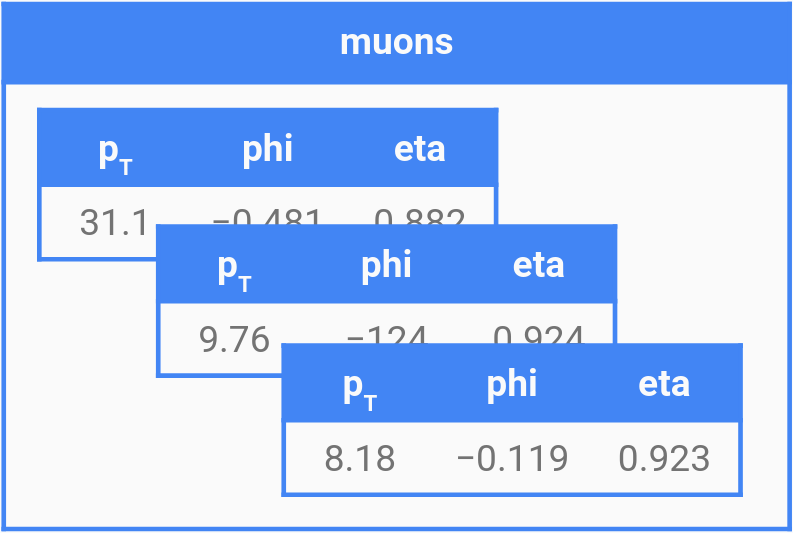
\includegraphics[width=\linewidth]{muons-as-objects.png}

\column{0.5\linewidth}
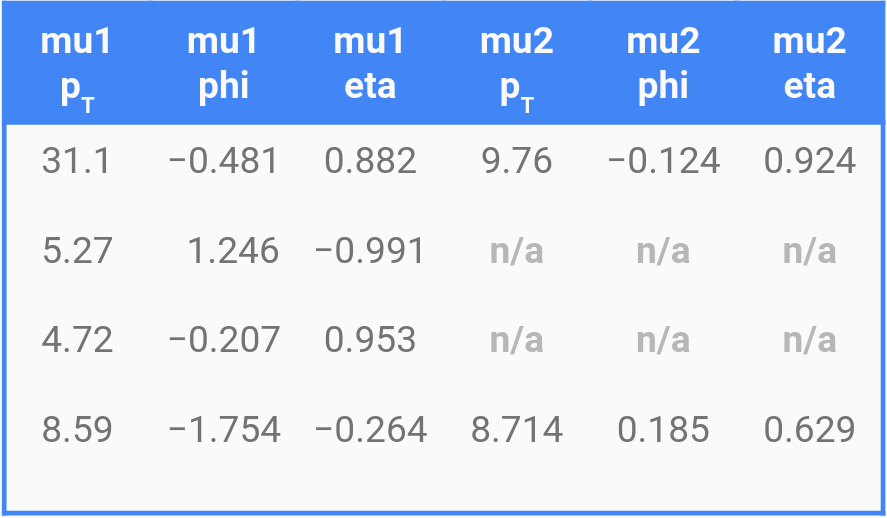
\includegraphics[width=\linewidth]{muons-as-a-table.png}
\end{columns}

\begin{uncoverenv}<2>
\vspace{0.25 cm}
Analysis datasets are big lists of variable-length lists of structs/objects/records.

\vspace{0.25 cm}
\scriptsize
\begin{Verbatim}[commandchars=\\\{\}]
[[Muon(\textcolor{darkgreen}{31.1}, \textcolor{darkorange}{-0.481}, \textcolor{blue}{0.882}), Muon(\textcolor{darkgreen}{9.76}, \textcolor{darkorange}{-0.124}, \textcolor{blue}{0.924}), Muon(\textcolor{darkgreen}{8.18}, \textcolor{darkorange}{-0.119}, \textcolor{blue}{0.923})],
 [Muon(\textcolor{darkgreen}{5.27}, \textcolor{darkorange}{1.246}, \textcolor{blue}{-0.991})],
 [Muon(\textcolor{darkgreen}{4.72}, \textcolor{darkorange}{-0.207}, \textcolor{blue}{0.953})],
 [Muon(\textcolor{darkgreen}{8.59}, \textcolor{darkorange}{-1.754}, \textcolor{blue}{-0.264}), Muon(\textcolor{darkgreen}{8.714}, \textcolor{darkorange}{0.185}, \textcolor{blue}{0.629})],
 ...
\end{Verbatim}
\end{uncoverenv}
\end{frame}

\begin{frame}[fragile]{Columnar representation}
\vspace{0.5 cm}

But they don't have to be ``structs,'' pointers to contiguous $p_T$, $\eta$, $\phi$ triples.

\scriptsize
\begin{Verbatim}[commandchars=\\\{\}]
[[Muon(\textcolor{darkgreen}{31.1}, \textcolor{darkorange}{-0.481}, \textcolor{blue}{0.882}), Muon(\textcolor{darkgreen}{9.76}, \textcolor{darkorange}{-0.124}, \textcolor{blue}{0.924}), Muon(\textcolor{darkgreen}{8.18}, \textcolor{darkorange}{-0.119}, \textcolor{blue}{0.923})],
 [Muon(\textcolor{darkgreen}{5.27}, \textcolor{darkorange}{1.246}, \textcolor{blue}{-0.991})],
 [Muon(\textcolor{darkgreen}{4.72}, \textcolor{darkorange}{-0.207}, \textcolor{blue}{0.953})],
 [Muon(\textcolor{darkgreen}{8.59}, \textcolor{darkorange}{-1.754}, \textcolor{blue}{-0.264}), Muon(\textcolor{darkgreen}{8.714}, \textcolor{darkorange}{0.185}, \textcolor{blue}{0.629})],
 ...
\end{Verbatim}
\normalsize

\vspace{0.5 cm}
They can be contiguous by field with \only<1>{\textcolor{red}{counts}}\only<2,3,4>{counts} or \only<2>{\textcolor{red}{offsets}}\only<1,3,4>{offsets} or \only<3>{\textcolor{red}{starts/stops}}\only<1,2,4>{starts/stops} or \only<4>{\textcolor{red}{parents}}\only<1,2,3>{parents} arrays.

\vspace{0.25 cm}
\begin{tabular}{r l}
\only<1>{\small \textcolor{red}{counts}  & \textcolor{red}{\tt\scriptsize \ \ \ \ \ 3,\ \ \ \ \ \ \ \ \ \ \ \ \ \ \ \ \ \ \ \ \ \ 1,\ \ \ \ \ \ 1,\ \ \ \ \ \ 2\ \ \ \ \ \ \ \ \ } \\}
\only<2>{\small \textcolor{red}{offsets} & \textcolor{red}{\tt\scriptsize \ \ \ \ \ 0,\ \ \ \ \ \ \ \ \ \ \ \ \ \ \ \ \ \ \ \ \ \ 3,\ \ \ \ \ \ 4,\ \ \ \ \ \ 5,\ \ \ \ \ \ \ 7} \\}
\only<4>{\small \textcolor{red}{parents} & \textcolor{red}{\tt\scriptsize \ \ \ \ \ 0,\ \ \ \ \ \ 0,\ \ \ \ \ \ 0,\ \ \ \ \ \ 1,\ \ \ \ \ \ 2,\ \ \ \ \ \ 3,\ \ \ \ \ 3} \\}
\only<3>{\small \textcolor{red}{starts}  & \textcolor{red}{\tt\scriptsize \ \ \ \ \ 0,\ \ \ \ \ \ \ \ \ \ \ \ \ \ \ \ \ \ \ \ \ \ 3,\ \ \ \ \ \ 4,\ \ \ \ \ \ 5\ \ \ \ \ \ \ \ \ } \\}
\uncover<3>{\small \textcolor{red}{stops}   & \textcolor{red}{\tt\scriptsize \ \ \ \ \ 3,\ \ \ \ \ \ \ \ \ \ \ \ \ \ \ \ \ \ \ \ \ \ 4,\ \ \ \ \ \ 5,\ \ \ \ \ \ 7\ \ \ \ \ \ \ \ \ } \\}
\small \mbox{\hspace{1 cm}$p_T$} & \textcolor{darkgreen}{\tt\scriptsize \ \ 31.1,\ \ \ 9.76,\ \ \ 8.18,\ \ \ 5.27,\ \ \ 4.72,\ \ \ 8.59, 8.714} \\
\small phi &  \textcolor{darkorange}{\tt\scriptsize -0.481,\ -0.123,\ -0.119,\ \ 1.246,\ -0.207,\ -1.754,\ 0.185} \\
\small eta &        \textcolor{blue}{\tt\scriptsize \ 0.882,\ \ 0.924,\ \ 0.923,\ -0.991,\ \ 0.953,\ -0.264,\ 0.629} \\
\end{tabular}
\end{frame}

\begin{frame}[fragile]{This allows for efficient ways of {\it manipulating} data}
\vspace{0.25 cm}

``Remove the first muon from each event.'' \uncover<2->{\textcolor{red}{$\longrightarrow$ rewrite all inner lists.}}

\scriptsize
\begin{onlyenv}<1>
\begin{Verbatim}[commandchars=\\\{\}]
[[Muon(\textcolor{darkgreen}{31.1}, \textcolor{darkorange}{-0.481}, \textcolor{blue}{0.882}), Muon(\textcolor{darkgreen}{9.76}, \textcolor{darkorange}{-0.124}, \textcolor{blue}{0.924}), Muon(\textcolor{darkgreen}{8.18}, \textcolor{darkorange}{-0.119}, \textcolor{blue}{0.923})],
 [Muon(\textcolor{darkgreen}{5.27}, \textcolor{darkorange}{1.246}, \textcolor{blue}{-0.991})],
 [Muon(\textcolor{darkgreen}{4.72}, \textcolor{darkorange}{-0.207}, \textcolor{blue}{0.953})],
 [Muon(\textcolor{darkgreen}{8.59}, \textcolor{darkorange}{-1.754}, \textcolor{blue}{-0.264}), Muon(\textcolor{darkgreen}{8.714}, \textcolor{darkorange}{0.185}, \textcolor{blue}{0.629})],
 ...
\end{Verbatim}
\end{onlyenv}\begin{onlyenv}<2->
\begin{Verbatim}[commandchars=\\\{\}]
[[     \textcolor{darkgreen}{    }  \textcolor{darkorange}{      }  \textcolor{blue}{     }   Muon(\textcolor{darkgreen}{9.76}, \textcolor{darkorange}{-0.124}, \textcolor{blue}{0.924}), Muon(\textcolor{darkgreen}{8.18}, \textcolor{darkorange}{-0.119}, \textcolor{blue}{0.923})],
 [     \textcolor{darkgreen}{    }  \textcolor{darkorange}{     }  \textcolor{blue}{      } ],
 [     \textcolor{darkgreen}{    }  \textcolor{darkorange}{      }  \textcolor{blue}{     } ],
 [     \textcolor{darkgreen}{    }  \textcolor{darkorange}{      }  \textcolor{blue}{      }   Muon(\textcolor{darkgreen}{8.714}, \textcolor{darkorange}{0.185}, \textcolor{blue}{0.629})],
 ...
\end{Verbatim}
\end{onlyenv}
\normalsize

\vspace{0.5 cm}
``Remove the first muon from each event.'' \uncover<2->{\textcolor{red}{$\longrightarrow$ increase all starts by 1.}}

\vspace{0.25 cm}
\begin{onlyenv}<1>
\begin{tabular}{r l}
\small starts  &                    {\tt\scriptsize \ \ \ \ \ 0,\ \ \ \ \ \ \ \ \ \ \ \ \ \ \ \ \ \ \ \ \ \ 3,\ \ \ \ \ \ 4,\ \ \ \ \ \ 5\ \ \ \ \ \ \ \ \ } \\
\small stops   &                    {\tt\scriptsize \ \ \ \ \ 3,\ \ \ \ \ \ \ \ \ \ \ \ \ \ \ \ \ \ \ \ \ \ 4,\ \ \ \ \ \ 5,\ \ \ \ \ \ 7\ \ \ \ \ \ \ \ \ } \\
\small $p_T$ & \textcolor{darkgreen}{\tt\scriptsize \ \ 31.1,\ \ \ 9.76,\ \ \ 8.18,\ \ \ 5.27,\ \ \ 4.72,\ \ \ 8.59, 8.714} \\
\small phi &  \textcolor{darkorange}{\tt\scriptsize -0.481,\ -0.123,\ -0.119,\ \ 1.246,\ -0.207,\ -1.754,\ 0.185} \\
\small eta &        \textcolor{blue}{\tt\scriptsize \ 0.882,\ \ 0.924,\ \ 0.923,\ -0.991,\ \ 0.953,\ -0.264,\ 0.629} \\
\end{tabular}
\end{onlyenv}\begin{onlyenv}<2->
\begin{tabular}{r l}
\small starts  &     \textcolor{red}{\tt\scriptsize \ \ \ \ \ 1,\ \ \ \ \ \ \ \ \ \ \ \ \ \ \ \ \ \ \ \ \ \ 4,\ \ \ \ \ \ 5,\ \ \ \ \ \ 6\ \ \ \ \ \ \ \ \ } \\
\small stops   &                    {\tt\scriptsize \ \ \ \ \ 3,\ \ \ \ \ \ \ \ \ \ \ \ \ \ \ \ \ \ \ \ \ \ 4,\ \ \ \ \ \ 5,\ \ \ \ \ \ 7\ \ \ \ \ \ \ \ \ } \\
\small $p_T$ & \textcolor{darkgreen}{\tt\scriptsize \ \ 31.1,\ \ \ 9.76,\ \ \ 8.18,\ \ \ 5.27,\ \ \ 4.72,\ \ \ 8.59, 8.714} \\
\small phi &  \textcolor{darkorange}{\tt\scriptsize -0.481,\ -0.123,\ -0.119,\ \ 1.246,\ -0.207,\ -1.754,\ 0.185} \\
\small eta &        \textcolor{blue}{\tt\scriptsize \ 0.882,\ \ 0.924,\ \ 0.923,\ -0.991,\ \ 0.953,\ -0.264,\ 0.629} \\
\end{tabular}\end{onlyenv}

\vspace{0.5 cm}
\uncover<3>{We didn't need to touch any contents (read them from disk, decompress them\ldots).}
\end{frame}

\begin{frame}{Library for manipulating non-standard array types}
\vspace{0.25 cm}
\begin{columns}
\column{0.45\linewidth}

\includegraphics[width=\linewidth]{awkward-logo.pdf}

\vspace{0.25 cm}
\hfill \scriptsize \textcolor{darkblue}{\mbox{\hspace{-0.75 cm}\url{https://github.com/scikit-hep/awkward-array}\hspace{-0.65 cm}}}

\column{0.55\linewidth}
\vspace{0.5 cm}
\vspace{2\baselineskip}
\begin{itemize}
\item variable-length subarrays: \textcolor{darkblue}{``jagged arrays''}
\item struct-of-arrays viewed as array-of-structs
\item nullable types
\item heterogeneous types (tagged unions)
\item cross-references or even cyclic references
\item sparse, non-contiguous, lazy
\end{itemize}

\vspace{0.5 cm}
\uncover<2>{\textcolor{darkblue}{Fully composable:} any awkward array can be placed within any other awkward array.}
\end{columns}
\end{frame}

\begin{frame}[fragile]{Not lacking for data types}
\vspace{0.5 cm}
Nullable, heterogeneous, multiple levels of depth, nested records\ldots

\small
\begin{minted}{python}
>>> import awkward
>>> array = awkward.fromiter(
...     [[1.1, 2.2, None, 3.3, None],
...      [4.4, [5.5]],
...      [{"x": 6, "y": {"z": 7}}, None, {"x": 8, "y": {"z": 9}}]])
\end{minted}

\begin{uncoverenv}<2->
\begin{minted}{python}
>>> print(array)            # internally, these are all arrays
[[1.1 2.2 None 3.3 None] [4.4 [5.5]] [<Row 0> None <Row 1>]]
\end{minted}
\end{uncoverenv}

\begin{uncoverenv}<3->
\begin{minted}{python}
>>> print(array[:, -2:])    # all of outer list, last two of inner
[[3.3 None] [4.4 [5.5]] [None <Row 1>]]
\end{minted}
\end{uncoverenv}

\begin{uncoverenv}<4->
\begin{minted}{python}
>>> (array + 100).tolist()  # element-wise function applied to arrays
[[101.1, 102.2, None, 103.3, None],
 [104.4, [105.5]],
 [{'x': 106, 'y': {'z': 107}}, None, {'x': 108, 'y': {'z': 109}}]]
\end{minted}
\end{uncoverenv}
\end{frame}

\begin{frame}{Columnar data structures minimize memory use and time}
\vspace{0.5 cm}
One operation, deriving $p_z$ of a variable number of $p_T$ and $\eta$ per event, using \textcolor{darkorange2}{awkward-array}, \textcolor{blue}{ROOT}, \textcolor{darkpink}{pure Python}, and \textcolor{darkgreen}{root\_numpy}.

\vspace{0.2 cm}
\begin{center}
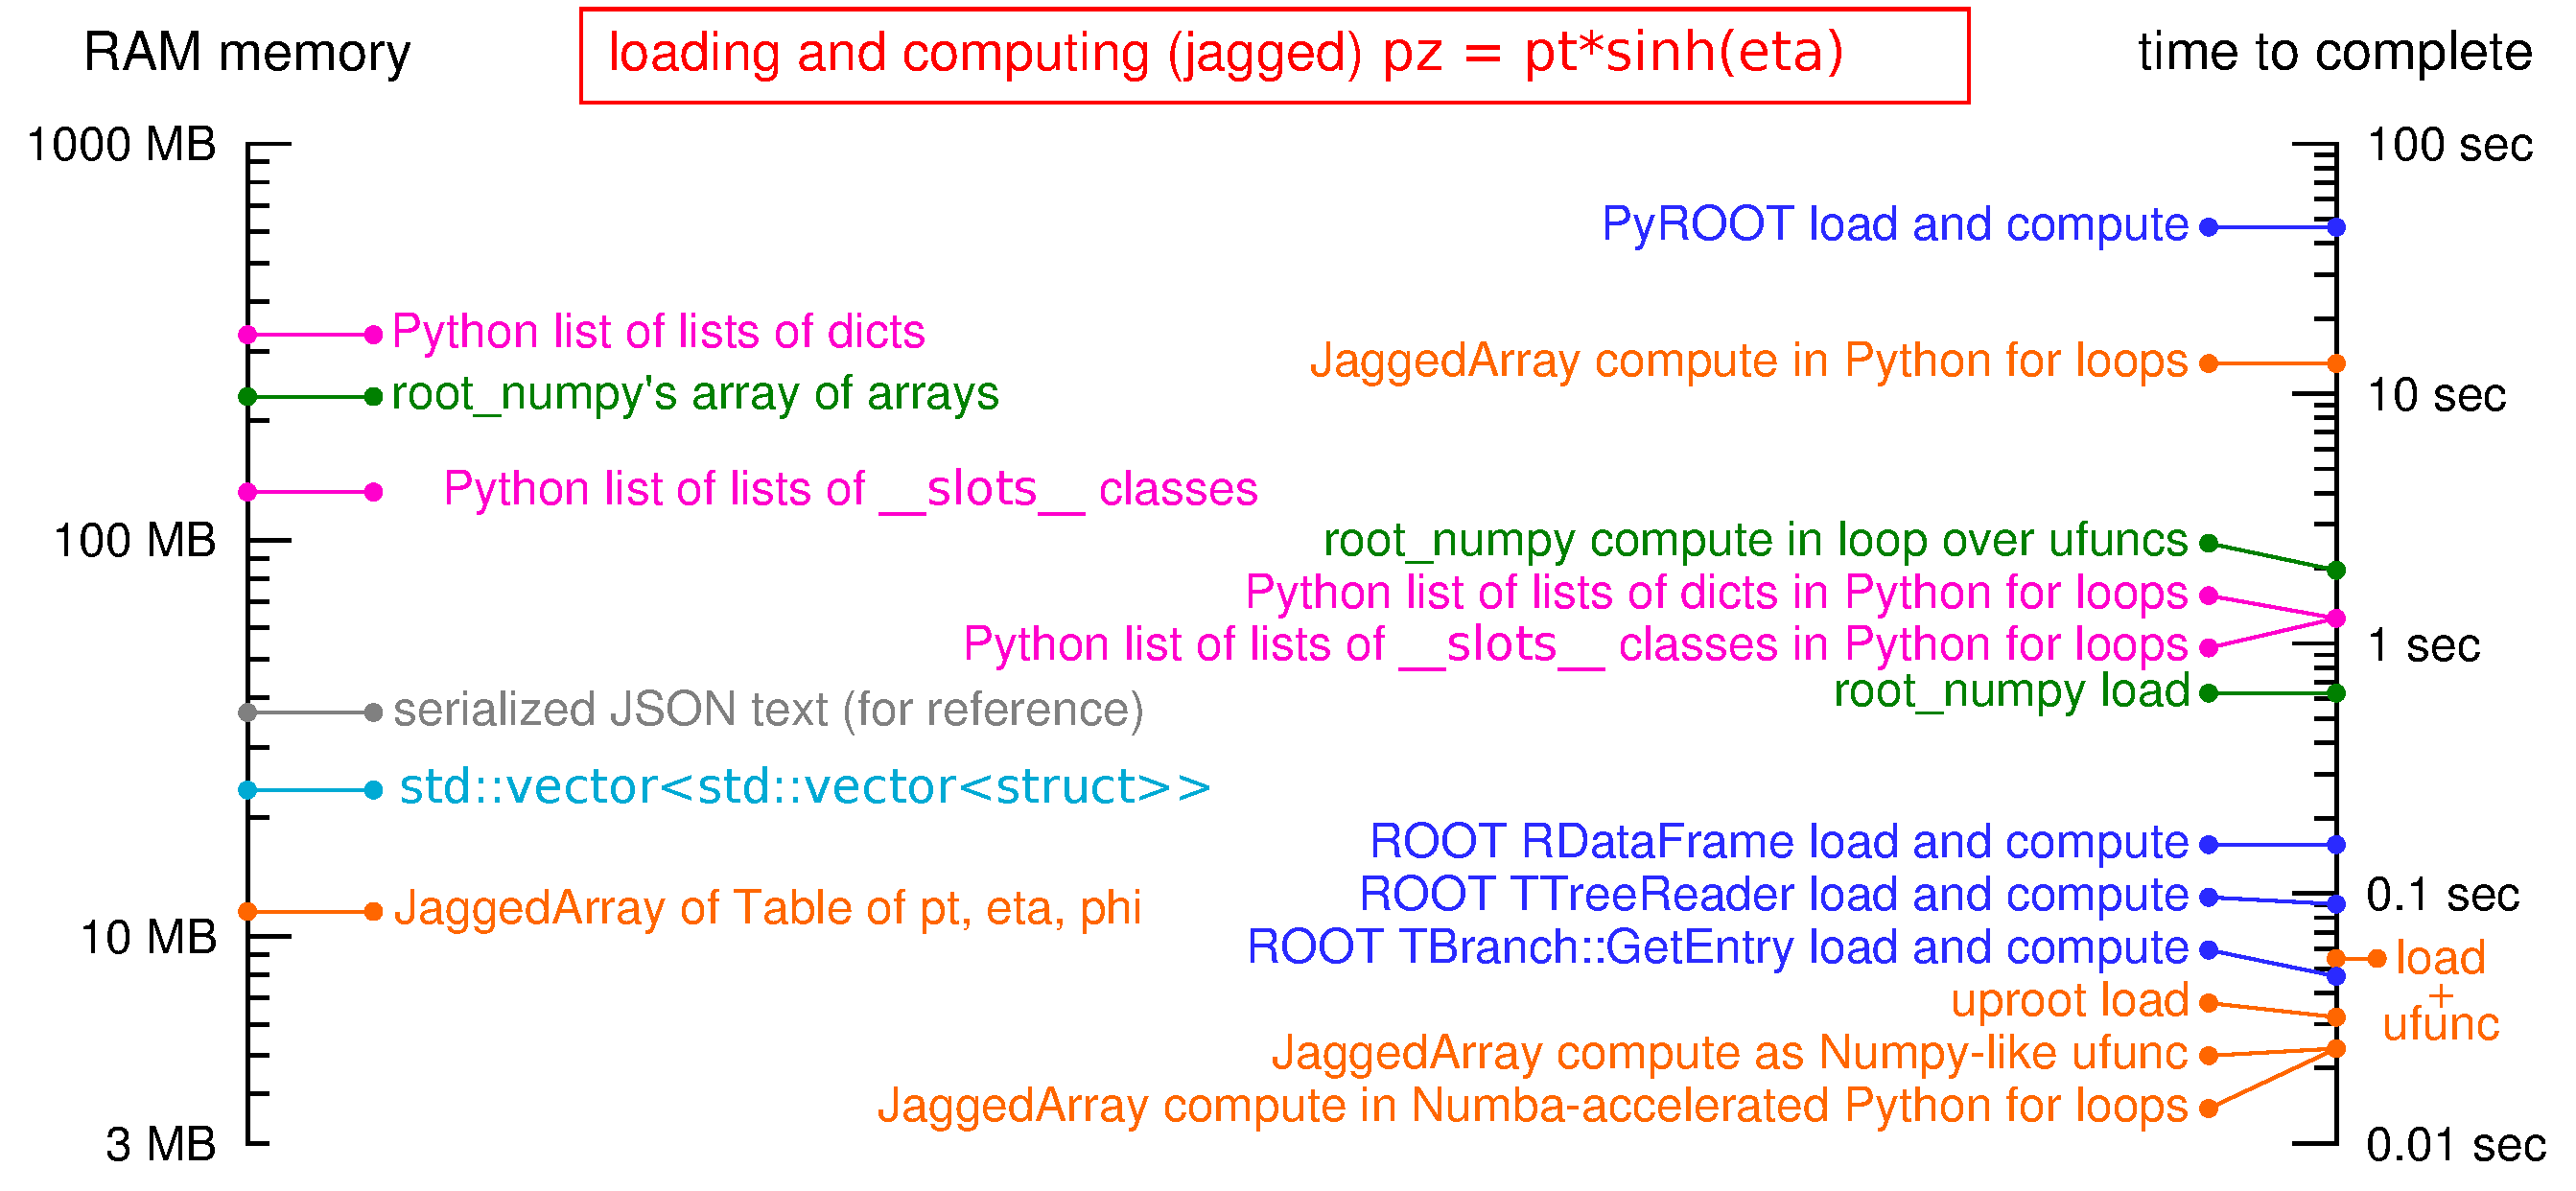
\includegraphics[width=0.9\linewidth]{logscales.pdf}
\end{center}
\end{frame}

\begin{frame}{Real life}
\vspace{0.5 cm}
\LARGE
\begin{center}
a single operation $\ne$ a physics analysis
\end{center}
\end{frame}

\begin{frame}{Beyond toy studies}
\vspace{0.5 cm}
\begin{columns}
\column{0.2\linewidth}

\includegraphics[width=\linewidth]{coffea-logo.png}

\column{0.8\linewidth}
\hspace{-0.2 cm}\Huge Coffea

\vspace{0.25 cm}
\large {\bf C}olumnar {\bf O}bject {\bf F}ramework {\bf F}or {\bf E}fficient {\bf A}nalysis

\vspace{0.25 cm}
\normalsize Matteo~Cremonesi, Lindsey~Gray, Oliver~Gutsche, Allison~Hall, Bo~Jayatilaka, Igor~Mandrichenko, Kevin~Pedro, Nick~Smith~[FNAL], and~me~[Princeton] \hfill \textcolor{blue}{\url{https://github.com/CoffeaTeam}}
\end{columns}

\begin{center}
\begin{minipage}{0.8\linewidth}
\large Performing two complete CMS analyses with columnar tools:
\begin{itemize}
\item Dark Higgs search
\item Boosted SM $H \to b\bar{b}$
\end{itemize}
\end{minipage}
\end{center}

\vspace{0.25 cm}
Also developing {\tt fnal-column-analysis-tools}, a HEP layer on awkward-array,
and a distributed query processing system with Ben Galewsky, Mark Neubauer [Illinois], and Andrew Melo [Vanderbilt].
\end{frame}

\begin{frame}[fragile]{First finished analysis: $Z$ peak}
\vspace{0.5 cm}
$Z$ peak is the ``hello world'' of analysis frameworks.

\vspace{0.5 cm}
\textcolor{darkblue}{This implementation is realistic:} run-lumi mask, pile-up correction, ID scale factors, and $ee$/$\mu\mu$/$e\mu$ channels. 350~lines in a Jupyter notebook, accessing 25 columns.

\vspace{0.25 cm}
\begin{columns}
\column{0.4\linewidth}
\large
\begin{description}
\item[columnar analysis:] \hfill \mbox{\hspace{-1 cm}6~$\mu$s/event/thread (165~kHz)}
\item[ROOT C++:] \hfill \mbox{\hspace{-1 cm}4~$\mu$s/event/thread (250~kHz)}
\end{description}

\vspace{0.25 cm}
Columnar analysis is about 50\% slower than its C++ equivalent.

\column{0.4\linewidth}
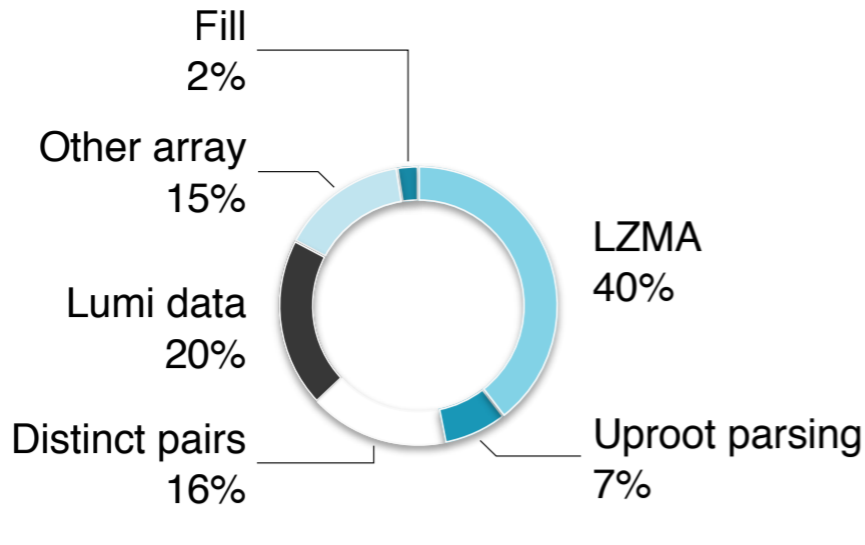
\includegraphics[width=\linewidth]{zpeak-performance-breakdown.png}
\end{columns}
\end{frame}

\begin{frame}{Second near-complete analysis}
\vspace{0.5 cm}
\begin{columns}[t]
\column{0.4\linewidth}
\textcolor{darkblue}{Prototype of boosted $H \to b\bar{b}$ has}
\begin{itemize}
\item recursive gen parent-finding
\item gen-reco matching
\item binned corrections
\item parametric corrections
\item systematics
\end{itemize}

\large
\vspace{0.25 cm}
70~$\mu$s/event/thread (14~kHz)

\vspace{0.25 cm}
Uses about 100 columns.
\end{columns}
\end{frame}

\begin{frame}[fragile]{Analyst's ``favorite stanzas'' of the boosted $H \to b\bar{b}$ analysis}
\vspace{0.5 cm}
%% \textcolor{darkblue}{\hspace{-0.15 cm}Example of combinatorics: gen-reco matching}

%% \small
%% \begin{minted}{python}
%% # make an array of all gen-reco pairs
%% pairing = gen.cross(reco, nested=True)

%% # delta R between gen (i0) and reco (i1)
%% metric = delta_r(pairing.i0, pairing.i1)

%% # the smallest delta R is best (indexes)
%% best = metric.argmin()

%% # but keep only delta R < 0.5 (mask)
%% passes_cut = (metric[best] < 0.5)

%% # now apply indexes and mask to select
%% selected_pair = pairing[best][passes_cut]
%% genrecos = selected_pair.flatten(axis=1)
%% \end{minted}
\begin{columns}
\column{0.8\linewidth}
\textcolor{darkblue}{VBF signal region definition:}

\scriptsize
\begin{minted}{python}
AK4jet_AK8jet_matches = ak4_goodjets.fastmatch(leadingak8jet)
unmatched_ak4    = ak4_goodjets[~AK4jet_AK8jet_matches]
vbf_ak4_pairs    = unmatched_ak4.p4.distincts(nested=True)
vbf_ak4_detas    = np.abs(vbf_ak4_pairs.i0.eta - vbf_ak4_pairs.i1.eta).flatten()
vbf_ak4_maxdetas = vbf_ak4_detas.argmax()
vbf_ak4_masses   = (vbf_ak4_pairs.i0 + vbf_ak4_pairs.i1).mass.flatten()[vbf_ak4_maxdetas]
vbf_ak4_pass     = (vbf_ak4_detas[vbf_ak4_maxdetas] > 3.25) & (vbf_ak4_masses > 975.0)
\end{minted}
\column{0.2\linewidth}
\end{columns}

\normalsize

\vspace{0.5 cm}
\begin{columns}
\column{0.2\linewidth}
\column{0.8\linewidth}
\textcolor{darkblue}{Leading fat-jet selection with vetos:}
\scriptsize
\begin{minted}{python}
k8puppijet_pt200 = ak8puppijet[
                       passLooseJetSel(ak8puppijet) & 
                       (ak8puppijet.pt > 200) & 
                       (np.abs(ak8puppijet.eta) < 2.5)]
ak8veto = ~(
    ak8puppijet_pt200.fastmatch(vetoMuons,deltaRCut=0.4) | 
    ak8puppijet_pt200.fastmatch(vetoElectrons,deltaRCut=0.4) |
    ak8puppijet_pt200.fastmatch(vetoPhotons,deltaRCut=0.4) )    
ak8jets_veto = ak8puppijet_pt200[ak8veto]    
leadingak8jet = ak8jets_veto[ak8jets_veto.pt.argmax()]
\end{minted}
\end{columns}
\end{frame}

\begin{frame}{Syntax is an extension of Numpy}
\vspace{0.25 cm}
\only<1>{\textcolor{red}{Numpy arrays must all be rectangular: vectors, matrices, and tensors.}}\only<2>{Numpy arrays must all be rectangular: vectors, matrices, and tensors.} \only<1>{Awkward arrays reproduce this behavior in rectangular cases and generalize in jagged cases.}\only<2>{\textcolor{red}{Awkward arrays reproduce this behavior in rectangular cases and generalize in jagged cases.}}

\begin{onlyenv}<1>
\begin{itemize}\setlength{\itemsep}{0.15 cm}
\item Multidimensional slices: \tabto{5.5 cm}{\small \mintinline{python}{rgb_pixels[0, 50:100, ::3]}}
\item Elementwise operations: \tabto{5.5 cm}{\small \mintinline{python}{all_pz = all_pt * sinh(all_eta)}}
\item Broadcasting: \tabto{5.5 cm}{\small \mintinline{python}{all_phi - 2*pi}}

\tabto{5.5 cm}\mbox{ }

\item Masking (list compaction): \tabto{5.5 cm}{\small \mintinline{python}{data[trigger & (pt > 40)]}}

\tabto{5.5 cm}\mbox{ }

\item Fancy indexing (gather/scatter): \tabto{5.5 cm}{\small \mintinline{python}{all_eta[argsort(all_pt)]}}

\tabto{5.5 cm}\mbox{ }

\item Row/column commutativity \tabto{5.5 cm}{\small \mintinline{python}{table["column"][7]} (row 7 of column array)}

(hides AoS $\leftrightarrow$ SoA): \tabto{5.5 cm}{\small \mintinline{python}{table[7]["column"]} (field of row tuple 7)}

\tabto{5.5 cm}\mbox{ }

\item Array reduction: \tabto{5.5 cm}{\small \mintinline{python}{array.sum()}} $\to$ scalar
\end{itemize}
\end{onlyenv}\begin{onlyenv}<2>
\begin{itemize}\setlength{\itemsep}{0.15 cm}
\item Multidimensional slices: \tabto{5.5 cm}{\small \mintinline{python}{events["jets"][:, 0]}} $\to$ first jet per event
\item Elementwise operations: \tabto{5.5 cm}{\small \mintinline{python}{jetpt * sinh(jeteta)}} $\to$ \mbox{keep jagged structure\hspace{-1 cm}}
\item Broadcasting: \tabto{5.5 cm}{\small \mintinline{python}{jetphi - metphi}} $\to$ expand {\small \mintinline{python}{metphi}} from

\tabto{5.5 cm}one-per-event to one-per-jet before operation

\item Masking (list compaction): \tabto{5.5 cm}{\small \mintinline{python}{data[trigger]}} $\to$ drop whole events

\tabto{5.5 cm}{\small \mintinline{python}{data[jetpt > 40]}} $\to$ drop jets from events

\item Fancy indexing (gather/scatter): \tabto{5.5 cm}{\small \mintinline{python}{a = argmax(jetpt)}} $\to$ \mbox{\small \mintinline{python}{[[2], [], [1], [4]]}\hspace{-0.5 cm}}

\tabto{5.5 cm}{\small \mintinline{python}{jeteta[a]}} $\to$ \mbox{\small \mintinline{python}{[[3.6], [], [-1.2], [0.4]]}\hspace{-0.5 cm}}

\item Row/column commutativity \tabto{5.5 cm}{\small \mintinline{python}{events["jets"]["pt"][7, 1]}},

(hides AoS $\leftrightarrow$ SoA): \tabto{5.5 cm}{\small \mintinline{python}{events["jets"][7]["pt"][1]}},

\tabto{5.5 cm}{\small \mintinline{python}{events[7]["jets"]["pt"][1]}}, \ldots

\item Jagged array reduction: \tabto{5.5 cm}{\small \mintinline{python}{jetpt.max()}} $\to$ array of max jet $p_T$ per event
\end{itemize}
\end{onlyenv}
\end{frame}

\begin{frame}[fragile]{Structure for most physics data: multiple candidates per event}
\vspace{0.4 cm}

\begin{center}
{\tt \small \textcolor{blue}{JaggedArray}(\textcolor{darkorange}{ObjectArray}(\textcolor{darkgreen}{Table}(px, py, pz, E), \textcolor{darkorange}{LorentzVector}))}
\end{center}

\begin{uncoverenv}<2->
\begin{itemize}
\item {\tt \small px}, {\tt \small py}, {\tt \small pz}, {\tt \small E} are flat Numpy arrays (all particles, all events).
\item \textcolor{darkgreen}{\tt \small Table} to present contiguous columns as an array of rows
\item \textcolor{darkorange}{\tt \small ObjectArray} to interpret rows of the \textcolor{darkgreen}{\tt \small Table} as \textcolor{darkorange}{\tt \small LorentzVector} objects
\item \textcolor{blue}{\tt \small JaggedArray} because there's a variable number of \textcolor{darkorange}{\tt \small LorentzVectors} per event
\end{itemize}
\end{uncoverenv}

\begin{uncoverenv}<3->
\vspace{0.5 cm}
Individual \textcolor{darkorange}{\tt \small LorentzVector} objects have kinematic methods---{\tt \small pt}, {\tt \small eta}, {\tt \small mass}, etc.--- but so do the \textcolor{darkorange}{\tt \small ObjectArray} and \textcolor{blue}{\tt \small JaggedArray}. Whole-array methods are vectorized.

\vspace{0.25 cm}
To compute the mass of all particles in all events are pack it into per-event sublists, you say

\small\begin{minted}{python}
>>> particles.mass
\end{minted}
\end{uncoverenv}
\end{frame}

\begin{frame}[fragile]{Putting it all together: a simple Z peak}
\small
\vspace{0.1 cm}
\begin{columns}
\column{1.1\linewidth}
\begin{minted}{python}
>>> import uproot
>>> dataset = uproot.open("HZZ-objects.root")["events"]
>>> array = dataset.array("muonp4")
\end{minted}

\begin{uncoverenv}<2->
\begin{minted}{python}
>>> array                                # muons for all events
<JaggedArray [[TLorentzVector(-52.899, -11.655, -8.1608, 54.779)
               TLorentzVector(37.738, 0.69347, -11.308, 39.402)] ...]>
\end{minted}
\end{uncoverenv}

\begin{uncoverenv}<3->
\begin{minted}{python}
>>> array[0, 1]                          # second muon in first event
TLorentzVector(37.738, 0.69347, -11.308, 39.402)
\end{minted}
\end{uncoverenv}

\begin{uncoverenv}<4->
\begin{minted}{python}
>>> hastwo = (array.counts >= 2)         # to select at least two muons
>>> leading = array[hastwo, 0]           # mask and select first
>>> subleading = array[hastwo, 1]        # mask and select second
\end{minted}
\end{uncoverenv}

\begin{uncoverenv}<5->
\begin{minted}{python}
>>> candidates = leading + subleading    # Lorentz vector sum across all
>>> candidates.mass                      # compute mass for all
array([90.22779777, 74.74654928, ..., 85.44384208, 75.96066262])
\end{minted}
\end{uncoverenv}
\end{columns}
\end{frame}

\begin{frame}[fragile]{Feedback from physicists}
\vspace{0.5 cm}\large
\begin{itemize}\setlength{\itemsep}{0.3 cm}
\item<1-> Many bug-fixes, of course.
\item<2-> {\tt\small argmin()} was an analysis bottleneck. Reimplemented to be 125$\times$ faster.
\item<3-> Validity checks (e.g.\ to ensure that all {\tt \small starts}/{\tt \small stops} are within {\tt \small content}) are expensive. Need to avoid redundant checks without removing safety.
\item<4-> Discovering which operations are frequently used in analysis, which aren't.
\item<5-> \textcolor{darkblue}{Interesting mistake:} analysts must unlearn order-dependent coding habits!

\small\begin{minted}{python}
(nMuons > 0) & (Muons_pt[:, 0] > 30) # intersection of masks
\end{minted}
\large

The latter might try to access the first of zero muons.

\vspace{0.25 cm}
\begin{uncoverenv}<6->
\textcolor{darkblue}{Instead,}

\small\begin{minted}{python}
Muons_pt[(nMuons > 0), 0] > 30       # mask first dim, pick 0
\end{minted}
\end{uncoverenv}
\end{itemize}
\end{frame}

\begin{frame}{Is this making analysis \underline{easier}?}
\vspace{0.5 cm}
\Large

\begin{center}
\begin{minipage}{0.8\linewidth}
\textcolor{darkblue}{If yes,} great! Continue developing array operations, thinking about their ``ergonomics,'' and optimize their implementations.

\vspace{0.75 cm}
\textcolor{darkblue}{If no,} it's still a useful abstraction layer, but we'll need a more user-friendly interface on top of it, such as a functional or declarative language.
\end{minipage}
\end{center}
\end{frame}

\begin{frame}{Half-hour interviews with physicists about array syntax}
\vspace{0.5 cm}
2 beginning grad students, 1 beginning and 1 advanced postdoc, 1 advanced researcher

\vspace{0.5 cm}
Everyone had most experience in C++ (5~years to decades), less in Python, which was primarily PyROOT (6~months to 3--4 years), very little in Numpy (2~to~5 months).

\vspace{0.5 cm}

\begin{onlyenv}<1>
\textcolor{darkblue}{Some motivated by execution speed, some by ease of use.}
\small
\begin{itemize}
\item ``Thirty minutes is too long to wait for a plot.''
\item ``Will be run order of a hundred times over the course of the year; this is a big investment.'' but ``For something that could be two times faster, I wouldn't do these optimizations.''
\item ``Ease of use is paramount; I've always struggled with poorly written code.'' and \\ ``Making it fast to run it again and again is {\it going around} ease of use.''
\item ``Ease of use is most important, even if execution speed decreases.''
\end{itemize}
\vspace{0.5 cm}
\end{onlyenv}

\begin{onlyenv}<2>
\textcolor{darkblue}{Some found it easier, some more difficult.}
\small
\begin{itemize}
\item ``Way, way much easier than applying cuts with for loops.''
\item ``Surprised by how conceptually different you have to think about selections, combining objects.'' but ``Not good or bad, just surprising that it has a learning curve.''
\item ``Individual problems that have been much more difficult than expected.'' and \\ ``Translating `if' statements is where I get hung up.'' but \\ ``Not inherently harder; just harder now for those of us used to the `for' loop version.''
\end{itemize}
\vspace{1 cm}
\end{onlyenv}

\begin{onlyenv}<3>
\textcolor{darkblue}{One point came up multiple times: easier to \underline{read} than \underline{write}.}
\small
\begin{itemize}
\item ``The good thing is, once you figure it out, it's clear why it works. It's not magic, you just have to get the mapping right.''
\item ``If I ask a student to read my code, he'll be able to read it. But five minutes later, he'll try something similar and it won't work.''
\end{itemize}
\vspace{2 cm}
\end{onlyenv}
\end{frame}

\begin{frame}{Further developments}
\vspace{0.2 cm}
\begin{itemize}\setlength{\itemsep}{0.35 cm}
\item<1-> Numba is a JIT-compiler for Python, but only for statically typed data.

Awkward-array types are ``statically typed at runtime,'' so I'm extending Numba to recognize and JIT-compile them.

\vspace{0.1 cm}
\textcolor{darkblue}{This will permit fast (compiled), \underline{imperative} (for-loop style) calculations in Python.}

\item<2-> Possible Google Summer of Code project to add \textcolor{darkblue}{precompiled and/or CUDA} implementations, depending on the abilities and interests of the student.

\item<3-> Michael Hedges (Purdue) is developing \textcolor{darkblue}{Pandas extensions}, so that DataFrame columns can contain and operate on jagged data.

\item<4-> Giuseppe Cerati (Fermilab) is investigating the use of jagged arrays in C++, to write \textcolor{darkblue}{reconstruction algorithms that are equally efficient on CPUs and GPUs.}

\vspace{0.1 cm}
\textcolor{darkblue}{Status:} implemented track-propagation in Python and switched from CPU to GPU with from ``{\tt \small import numpy as np}'' $\to$ ``{\tt \small import cupy as np}''.

\vspace{0.1 cm}
Reimplemented in C++ using xtensor (Numpy clone for C++).
\end{itemize}
\end{frame}

\begin{frame}{Conclusions}
\large
\vspace{0.5 cm}
Awkward-array is a library for complex data, presented as arrays. Jagged arrays are the most important for HEP. \textcolor{gray}{(Perhaps the only type {\it necessary} for HEP?)}


\vspace{0.5 cm}
\textcolor{darkblue}{We're beyond single-operation tests; we're implementing complete analyses.}

Performance is within a factor of two of C++, and there's low-hanging fruit for improvements.

\vspace{0.5 cm}
Physicists find it hard to write, but easy to read.

\vspace{0.5 cm}
This is an open area of development with many paths to follow!
\end{frame}

\end{document}
